\subsection{Calculation of Orbital Elements}
This can convert state velocity vector into orbital elements and vice versa. The inputs are as follows
\begin{table}[H]
\centering
\begin{tabular}{@{}cl@{}}
\toprule
\multirow{2}{*}{Inputs} & State and Velocity Vectors            \\ \cmidrule(l){2-2} 
                                 & \multicolumn{1}{l}{Orbital Elements} \\ \midrule
\multicolumn{1}{r}{\multirow{2}{*}{Outputs}} & \multicolumn{1}{l}{Orbital Elements} \\ \cmidrule(l){2-2} 
\multicolumn{1}{r}{}           & State and Velocity Vectors            \\ \bottomrule
\end{tabular}\caption{Inputs and outputs for Calculation of Orbital Elements}
\end{table}
\begin{figure}[H]
\begin{floatrow}
\ffigbox{%
  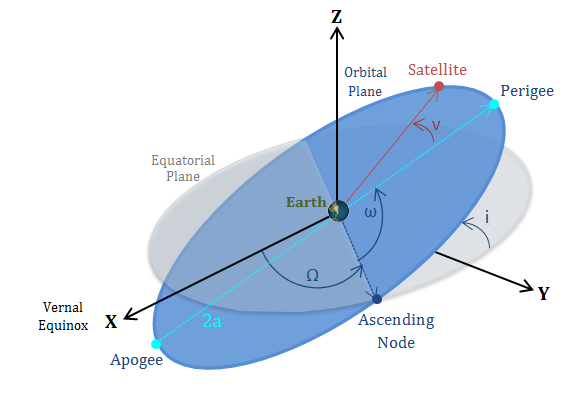
\includegraphics[scale=0.3]{images/COE.png}
}{
  \caption{Classical Orbital Elements} \label{COE}
}
\ffigbox{%
  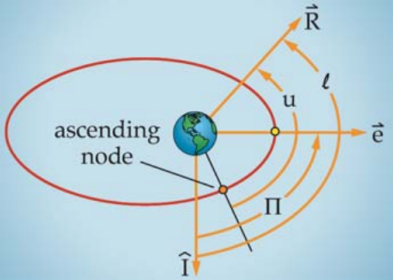
\includegraphics[scale=0.5]{images/AOE.png}
}{
  \caption{Alternate Orbital Elements} \label{AOE}
}
\end{floatrow}
\end{figure}

\subsection{2D and 3D Orbits}

Based on the inputs given the application can plot either 2D or 3D or both. If the inputs are just Semi major axis and eccentricity or Radius of perigee and apogee or, $r_1,\;v_1,\;\gamma_1$ then the resultant plot will be in the perifocal frame. If the inputs are state and velocity vector or orbital elements then the resultant will be a 3D orbit. 
\begin{table}[H]
\centering
\begin{tabular}{@{}cl@{}}
\toprule
\multirow{2}{*}{\textbf{Inputs}}                      & For 2D - $a,e/r_a,r_p/ r_1, v_1, \gamma_1$ \\ \cmidrule(l){2-2} 
                                             & For 3D - Orbital Elements, State Vectors   \\ \midrule
\multicolumn{1}{r}{\multirow{2}{*}{\textbf{Outputs}}} & Orbit in the Perifocal Frame               \\ \cmidrule(l){2-2} 
\multicolumn{1}{r}{}                         & Orbit in a virtual 3D Environment          \\ \bottomrule
\end{tabular}
\caption{I/O for 2D and 3D orbits}
\label{o23}
\end{table}
\subsection{Euler Angle}

The inputs for this are as in table(\ref{eadcm}). This code can be fed the model in 3D environment and the orientation of the model can be manipulated with this.
\begin{table}[H]
\centering
\begin{tabular}{@{}cl@{}}
\toprule
\multirow{2}{*}{\textbf{Inputs}}                      & Directional Cosine Matrix \\ \cmidrule(l){2-2} 
                                             & Euler Angles              \\ \midrule
\multicolumn{1}{r}{\multirow{2}{*}{\textbf{Outputs}}} & Euler Angles              \\ \cmidrule(l){2-2} 
\multicolumn{1}{r}{}                         & Directional Cosine Matrix \\ \bottomrule
\end{tabular}
\caption{I/O for conversion between Euler angle and DCM}
\label{eadcm}
\end{table}
\subsection{Sphere of Influence}
In this section, the user can either input the values or interact with the model in the 3D environment to see the corresponding output.
\begin{table}[H]
\centering
\begin{tabular}{@{}rl@{}}
\toprule
\multicolumn{1}{c}{\textbf{Inputs}} & Minor Body                     \\ \midrule
\multirow{2}{*}{\textbf{Outputs}}   & Radius of SOI in desired units \\ \cmidrule(l){2-2} 
                           & 3D visualization of sphere of influence in virtual environment                         \\ \bottomrule
\end{tabular}
\caption{I/O for Sphere of Influence}
\label{soi}
\end{table}
\subsection{Orbital Transfer}
This feature simulates the orbital transfer using various numerical methods. For now, this can perform Hohmann Transfer. The Inputs and outputs are as in table(\ref{tab:ot})
\begin{table}[H]
\centering
\begin{tabular}{@{}cl@{}}
\toprule
\multicolumn{1}{c}{\textbf{Inputs}} & Minor Body, Major Body, Orbital parameters of both initial and final orbit.                     \\ \midrule
\multirow{2}{*}{\textbf{Outputs}}   & Values such as Radius of apogee, Radius of perigee, DeltaV, Time-period of the orbit etc \\ \cmidrule(l){2-2} 
                           & 3D visualization of desired orbital transfer \\ \bottomrule
\end{tabular}
\caption{I/O for Orbital transfer}
\label{tab:ot}
\end{table}
\subsection{Calculation of Julian Day}
In this section the user can choose between Gregorian calendar and Julian calendar and with the other inputs they can obtain the Julian day of the corresponding date. 
\begin{table}[H]
\centering
\begin{tabular}{@{}cl@{}}
\toprule
\textbf{Inputs}  & YYYY-MM-DD , hh:mm:ss, Type of calender \\ \midrule
\textbf{Outputs} & Julian-day  \\ \bottomrule                                              
\end{tabular}
\caption{I/O for Julian-day}
\label{tab:jd}
\end{table}
\subsection{Calculation of Parameters of the Orbit}
The user can obtain various parameters by giving the details that they know of. If necessary they can plot the orbit too.
\begin{table}[H]
\centering
\begin{tabular}{@{}rl@{}}
\toprule
\multicolumn{1}{c}{\textbf{Inputs}} & $a,e/r_a, r_p/r_1,\;v_1,\;\gamma_1$/ Orbital Elements/State and velocity vectors \\ \midrule
\multirow{2}{*}{\textbf{Outputs}}   & $\mu,\;,h\;,\epsilon$, Forces and Velocity at significant position               \\ \cmidrule(l){2-2} 
                           & Mean Motion, Time Period                                                         \\ \bottomrule
\end{tabular}
\caption{I/O for Various Parameters of the Orbit}
\label{vpco}
\end{table}
\subsection{Sensitivity Analysis}
User has to select the type of calendar and the in the input section they have to select date and time and accuracy of digits and then by clicking on calculate button we will get Julian days in the output section. This takes in the required values an outputs how much of an error will that small change in the velocity or radius in the 3D environment.

\begin{table}[H]
\begin{tabular}{@{}cl@{}}
\toprule
\textbf{Input}  & State Vector, Velocity Vector and two delta-v with slight difference                                                                      \\ \midrule
\textbf{Output} & \begin{tabular}[c]{@{}l@{}}Percentage difference caused to the final orbit parameters due to slight \\ difference in delta-v\end{tabular} \\ \bottomrule
\end{tabular}\caption{I/O for Sensitivity Analysis}
\end{table}

\subsection{Position of One Spacecraft Relative To Another}
Based on the inputs of the user the relative velocity and orbit can be visualized in this section.
\begin{table}[H]
\begin{tabular}{@{}cl@{}}
\toprule
\textbf{Input}  & Major Body, State Vector and Velocity Vector of Minor Body    \\ \midrule
\textbf{Output} & Graph Showing the Minor bodies in the orbit around Major Body \\ \bottomrule
\end{tabular}\caption{I/O for Position of One Spacecraft Relative To Another}
\end{table}
\subsection{Lagrangian Points}
The Lagrangian points are points near two large orbiting bodies, the two objects exert an unbalanced gravitational force at a point, altering the orbit of whatever is at that point. At the Lagrange points, the gravitational forces of the two large bodies and the centrifugal force balance each other, The inputs and outputs are as follows.
\begin{table}[H]
\begin{tabular}{@{}cc@{}}
\toprule
\textbf{Input}  & Major Body, Minor Body and Distance Between them           \\ \midrule
\textbf{Output} & Lagrangian points polar coordinates and Graph showing them \\ \bottomrule
\end{tabular}\caption{I/O for Lagrangian Points}
\end{table}